%%% Local Variables:
%%% mode: latex
%%% TeX-master: "../main"
%%% coding: utf-8
%%% End:
% !TEX TS-program = pdflatexmk
% !TEX encoding = UTF-8 Unicode
% !TEX root = ../main.tex

This section discusses the findings and experience gained by implementing a project using \gls{WebGPU}. In addition, a comparison of the results is provided and possible future work is outlined.

The path tracer focuses on the given use case and is, therefore, not a general-purpose rendering engine. For example, it does not offer a physics engine, support for animations, or other features that are common in general-purpose rendering engines, such as \gls{Three.js}, \gls{Babylon.js}, or alternatives. Generally, the ray tracing technique is slower than rasterization-based approaches and is therefore not a silver bullet for all use cases. The results indicate that the developed path tracer is a viable option in the discussed use case of e-commerce.

\section{Comparison}

In order to contextualize the results, the presented work is compared to existing solutions. This includes a comparison to other open-source path tracers for the web, as well as a comparison to two alternative rendering strategies: web-based client-side real-time rendering using rasterization and offline ray-traced rendering.

\subsection*{Comparison to Prior Work}
\label{sec:comparisonToPriorWork}

The three open-source path tracers introduced in \autoref{sec:web-path-tracers} are alternatives to the renderer developed in this work. Comparing them based on quantitative measures such as \fGls{FPS}{\e{Frames per second}, measure of the rate at which consecutive images are rendered and displayed} is not meaningful as the number of samples required for high-fidelity renderings differs across the renderers. Nevertheless, defining a set of criteria to compare them is still possible.


\subsubsection*{WebGPU Support}

\gls{WebGPU} is a new technology and its support is likely to become more important in the future. The three alternatives currently do not support \gls{WebGPU} and still rely on \gls{WebGL}.

\subsubsection*{PBR Standard}

As discussed in \autoref{ch:materialDescriptionStandards}, a variety of standards exist for \gls{PBR}. While \gls{OpenPBR} is a new standard, it has already seen adoption by the industry and offers interoperability. \texttt{three-gpu-pathtracer} and \texttt{Three.js PathTracer} currently use custom \gls{PBR} standards or partially support \gls{glTF} \gls{PBR} extensions. \texttt{dspbr-pt} uses the \gls{DSPBR} standard.

\subsubsection*{Documentation}

For developers to use the library, the renderer should be well-documented. \texttt{strahl} and \texttt{three-gpu-pathtracer} provide documentation. \texttt{Three.js PathTracer} and \texttt{dspbr-pt} provide minimal documentation. None of the three alternatives provide a material editor.

\subsubsection*{Benchmark Setup}

A benchmark setup is important to assess the performance of the renderer. \texttt{strahl} provides a reproducible benchmark setup. None of the alternatives provide a comparable setup or measurements. This further complicates the comparison of the renderers.

\subsubsection*{Maintenance}

The availability of an \gls{npm} package can simplify the integration of the renderer into existing projects. Additionally, it enables updating libraries using a standardized process. \texttt{strahl}, \texttt{three-gpu-pathtracer}, and \texttt{dspbr-pt} provide an \gls{npm} package, while \texttt{Three.js PathTracer} does not. \texttt{strahl}, \texttt{three-gpu-pathtracer}, and \texttt{Three.js PathTracer} have been updated in 2024, while \texttt{dspbr-pt} has not been updated since 2022. Therefore, maintenance for \texttt{strahl} and \texttt{three-gpu-pathtracer} is provided while \texttt{Three.js PathTracer} and \texttt{dspbr-pt} are lacking in this regard.

\subsubsection*{Assessment}

\autoref{tab:rendererComparison} contains a high-level comparison between the four renderers. The renderer developed in this work is the only one that supports \gls{WebGPU} and uses the \gls{OpenPBR} standard. The extensive documentation and benchmark setup further distinguish the developed solution. Therefore, \texttt{strahl} provides an alternative to the existing renderers.

\begin{table}[H]
    \centering
    \ra{1.3}
    \begin{tabular}{@{}p{3cm}p{1.9cm}p{2.8cm}p{3.2cm}p{2.4cm}@{}}
    \toprule
     & \texttt{strahl} & \texttt{three-gpu-} \texttt{pathtracer} \cite{ThreeJsPathTracerJohnson} & \texttt{Three.js PathTracer} \cite{ThreeJsPathTracerLoftis} & \texttt{dspbr-pt} \cite{PathTracerDassault} \\
    \gls{WebGPU} \newline Support & Yes & No & No & No \\
    \gls{PBR} Standard & \gls{OpenPBR} & Custom & Custom & \gls{DSPBR} \\
    Documentation & yes & yes & minimal & minimal \\
    Benchmark Setup & yes & no & no & no \\
    Maintenance & provided & provided & lacking & lacking \\
    \bottomrule
    \end{tabular}
    \caption{High-level comparison between four open-source path tracers for the web.}
    \label{tab:rendererComparison}
  \end{table}

\subsection*{Comparison to Alternative Strategies}

The chosen architecture paradigm serves as an alternative to offline rendering solutions. In addition, the decision to implement ray tracing techniques contrasts with rasterization-based rendering engines. This section shows the comparison between these different options. For rasterization, \gls{Three.js} is used as an example, based on a minimal setup without pregenerated artifacts or advanced rendering techniques. For offline rendering, \fGls{RealityServer}{Platform for 3D rendering, which integrates the NVIDIA Iray global illumination rendering technology} renderings used by EAO are shown as a representative example. The three different renderings are visualized in \autoref{fig:final-rendering-comparison}.

\begin{figure}[H]
  \centering
  \begin{subfigure}[t]{0.3\textwidth}
    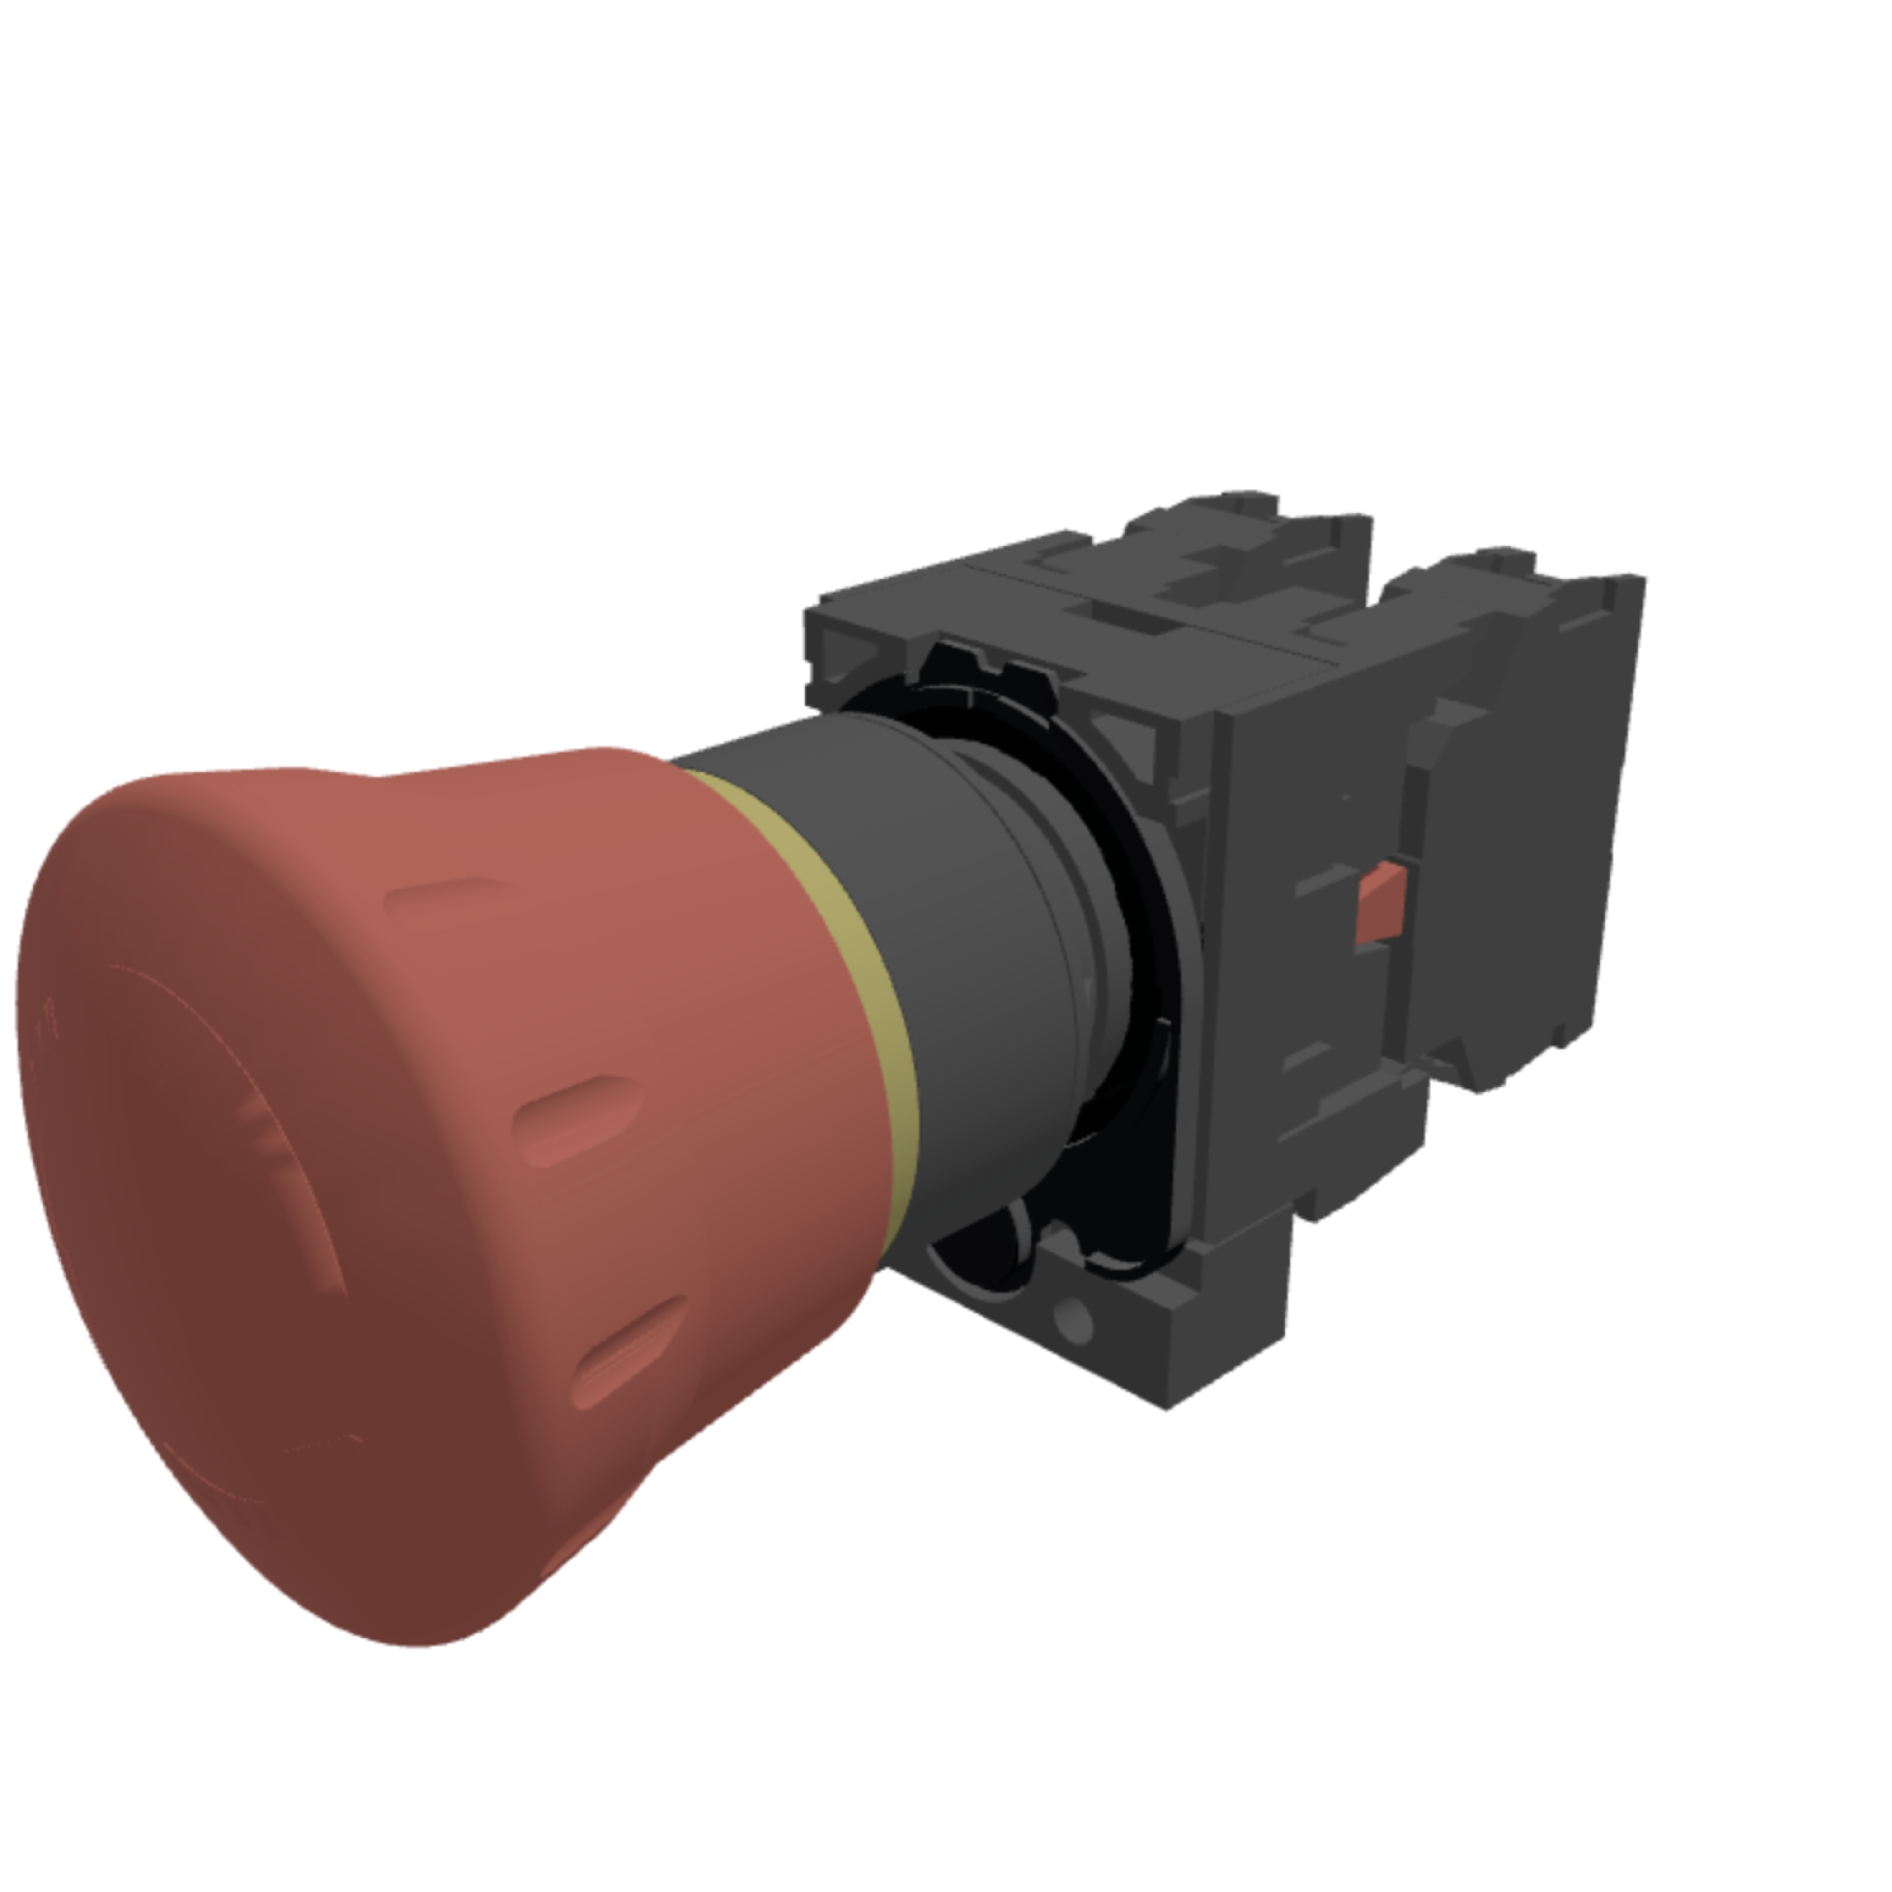
\includegraphics[width=\textwidth]{resources/comparison-three-js.png}
    \caption{Scene rendered by \gls{Three.js} using rasterization.}
    \label{fig:rasterization-rendering}
  \end{subfigure}
  \hfill
  \begin{subfigure}[t]{0.3\textwidth}
    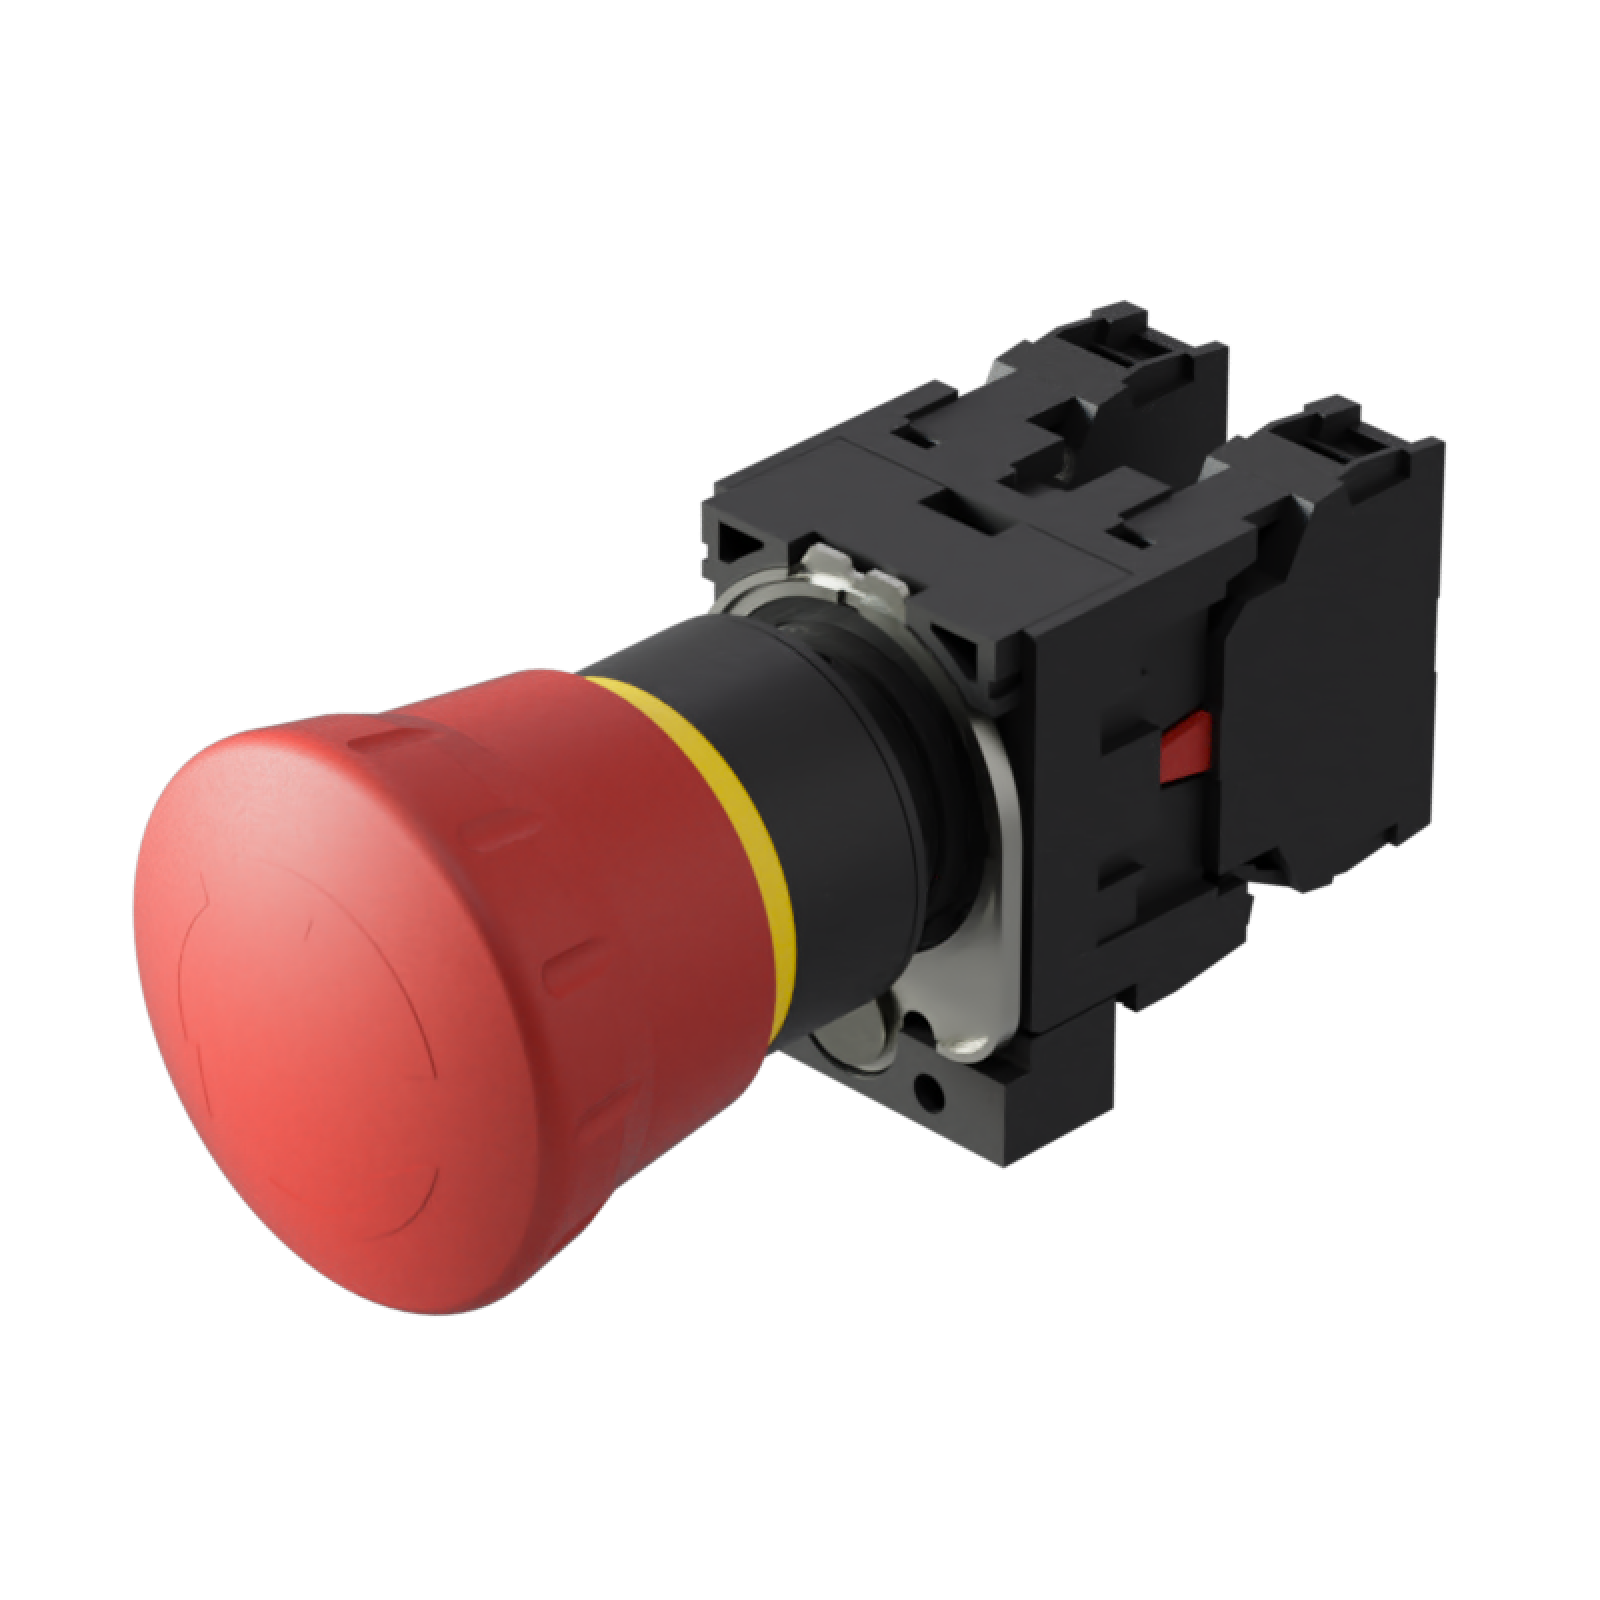
\includegraphics[width=\textwidth]{resources/comparison-offline-rendering.png}
    \caption{Offline rendering with \gls{RealityServer}, used by EAO \cite{eaoProductReference}.}
    \label{fig:offline-rendering}
  \end{subfigure}
  \hfill
  \begin{subfigure}[t]{0.3\textwidth}
    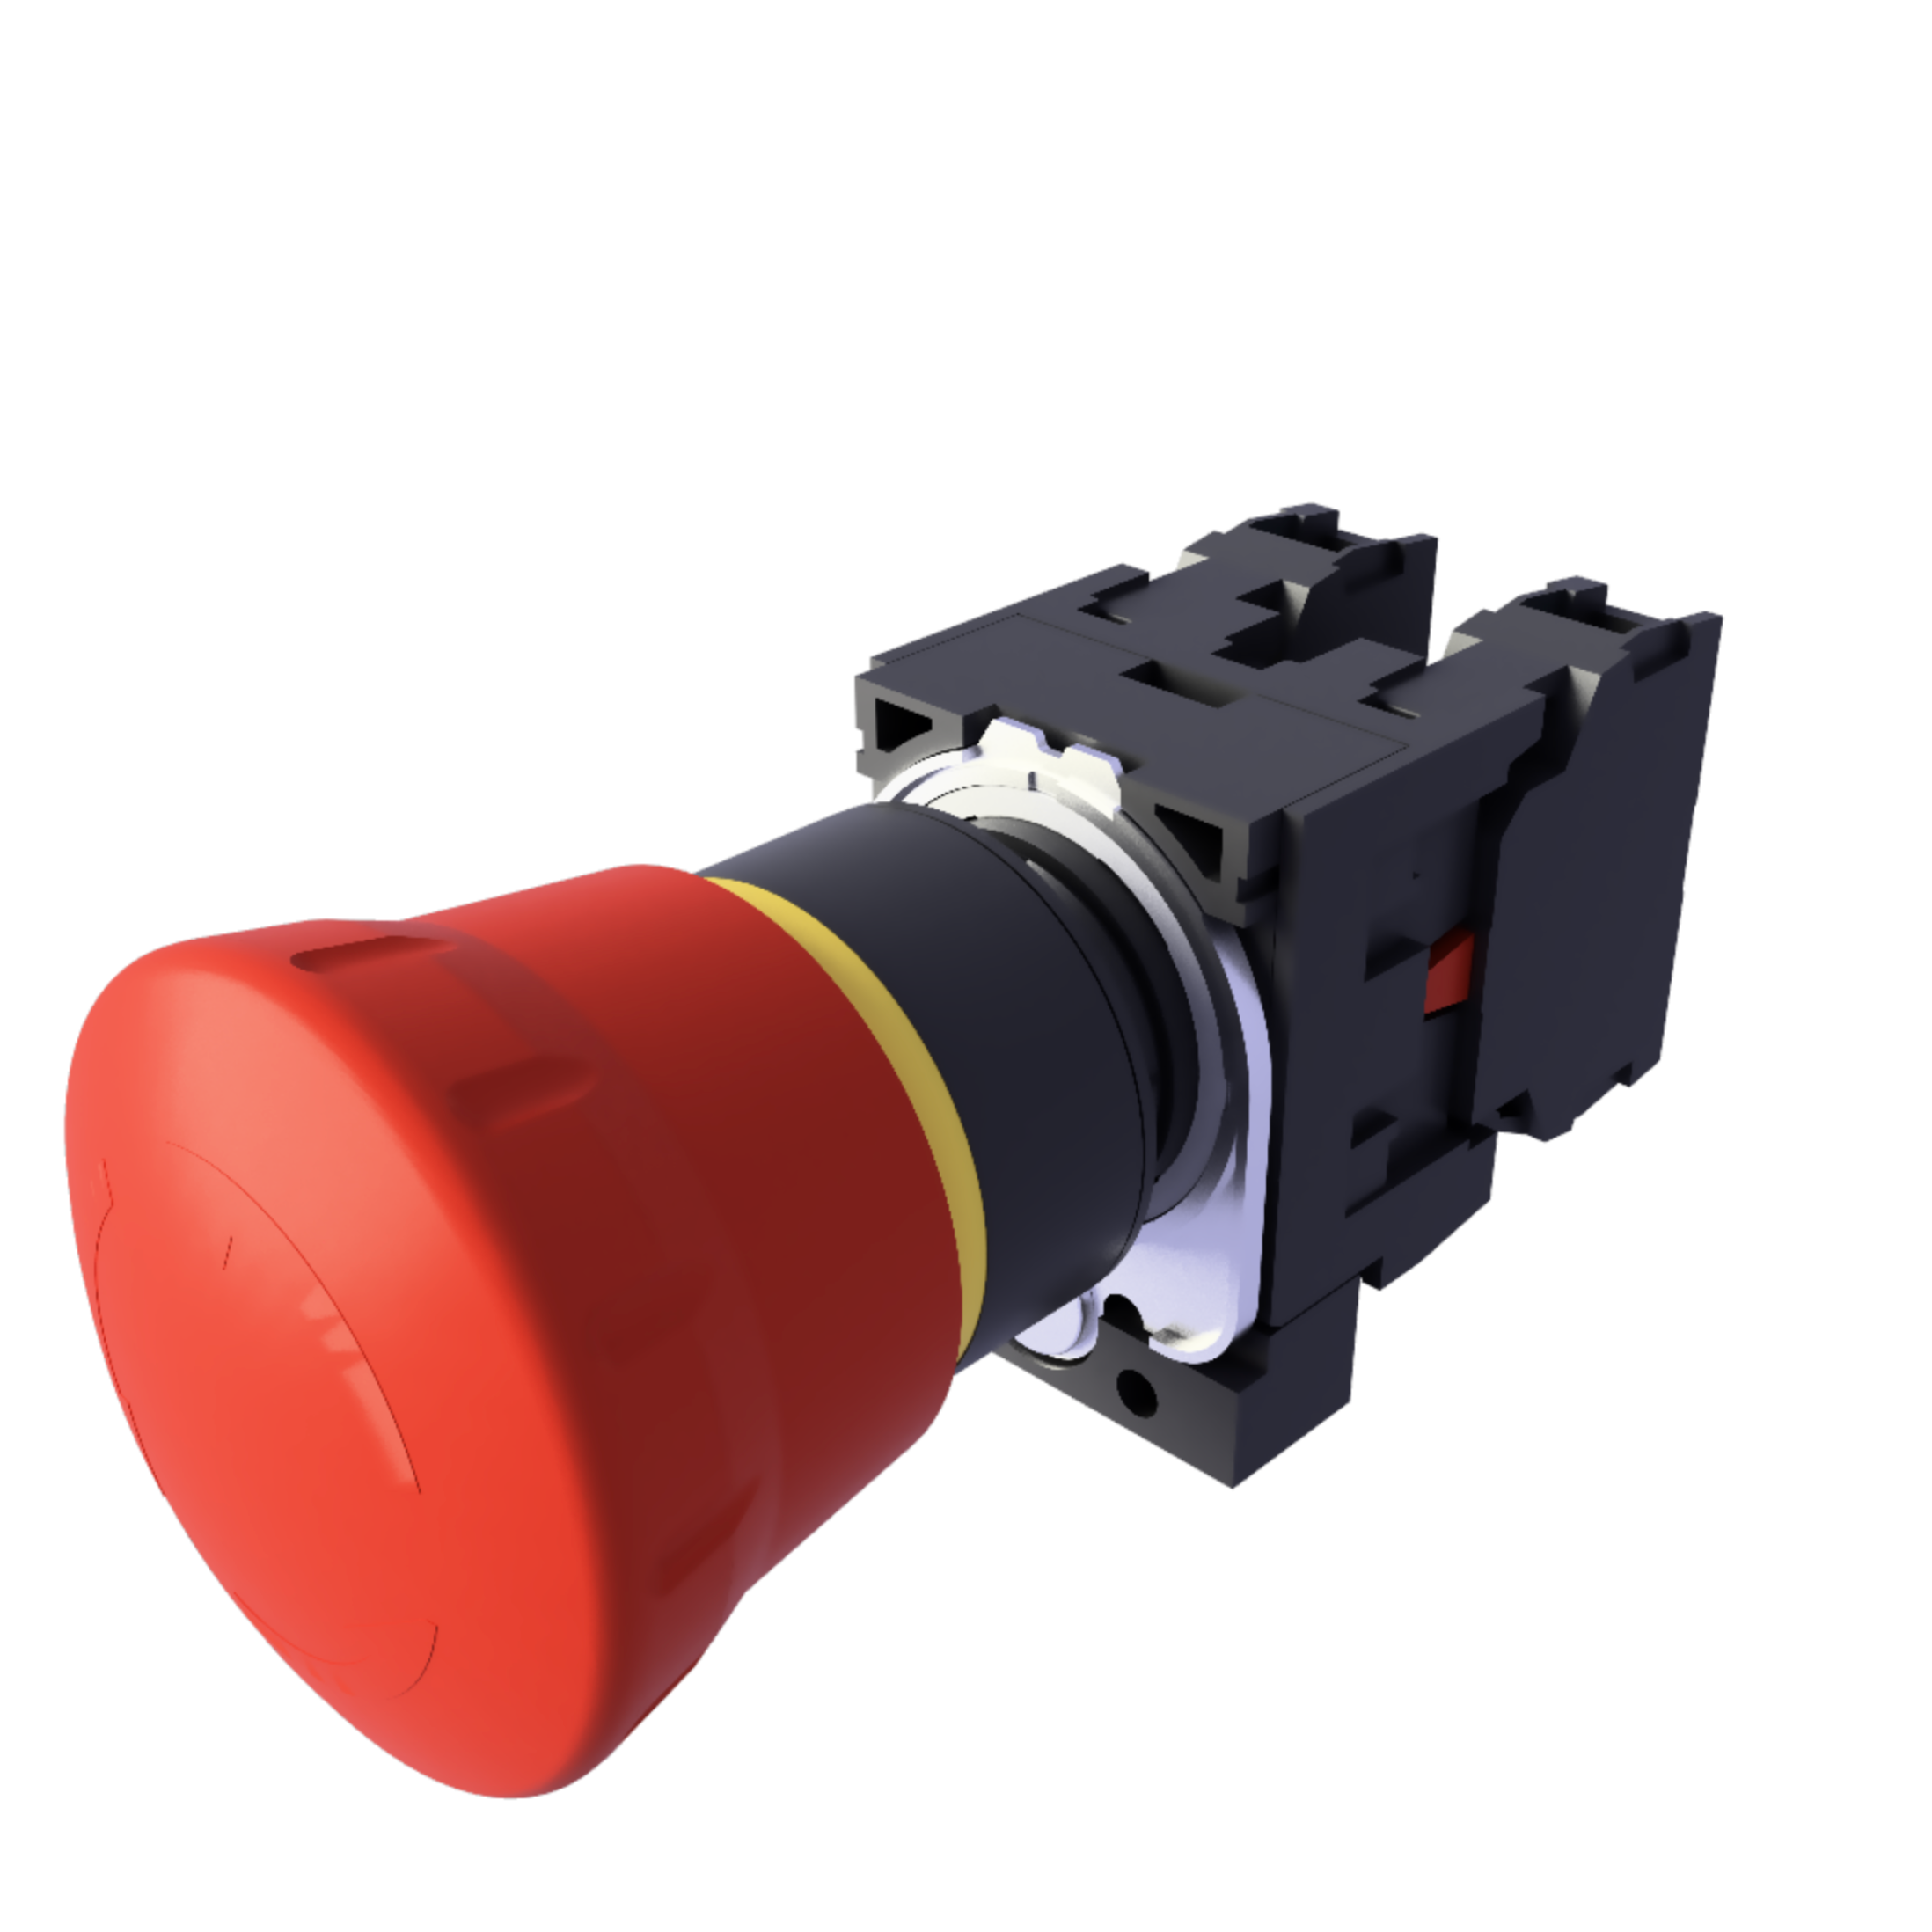
\includegraphics[width=\textwidth]{resources/comparison-strahl-rendering.png}
    \caption{Scene rendered with the developed path tracer.}
    \label{fig:strahl-rendering}
  \end{subfigure}
  \caption{Comparison of different rendering techniques.}
  \label{fig:final-rendering-comparison}
\end{figure}

Visually, differences in global illumination effects between the two ray-traced renderings and the rasterization rendering are apparent. Ambient occlusion on the terminal block is more pronounced in the ray-traced images. Reflection on the metal part is also more noticeable, and the surrounding environment is considered. Additionally, the shadows are more realistic and consider all light sources. The differences between the two ray-traced images are less apparent due to the similar rendering techniques. Certain differences, such as the color of the metal part and the reflection on the red part, are mainly due to changes in the material properties. This demonstrates the potential of the proposed solution to provide high-fidelity renderings in near real-time.

\section{Findings}

The main novelty introduced in this work is the development of a path tracer with \gls{WebGPU} using the \gls{OpenPBR} surface shading model. \gls{WebGPU} and \gls{OpenPBR} are promising endeavors for the future of 3D rendering, but as of 2024, they are relatively new and have yet to be widely adopted.

\subsection*{State of WebGPU}

\gls{WebGPU} is a promising technology for \gls{GPGPU} computations in the browser. The design reduces global state, enforces asynchrony, and is more explicit than \gls{WebGL}. However, to date, there are certain limitations regarding support and features.

\subsubsection*{Browser Support}

Due to the current state of support for \gls{WebGPU} in Safari and Mozilla Firefox, the production readiness of \gls{WebGPU} is still limited. Safari has announced plans to support \gls{WebGPU} and has launched a preview version \cite{SafariWebGPUSupport}. Firefox also has plans to support WebGPU \cite{FirefoxWebGPUSupport}. Thanks to the extensive conformance test suite \cite{WebGPUConformanceTestSuite}, it is more likely that the different implementations will be compatible with each other.

The main browser that supports \gls{WebGPU} to date is Chrome. \gls{WebGPU} has shipped to general use on desktops in May of 2023 \cite{ChromeWebGPUSupport}. Since January 2024, \gls{WebGPU} is also supported on modern Android devices \cite{ChromeAndroidWebGPUSupport}.

This means that using \gls{WebGPU} is straightforward on most modern devices, with the notable exception of Apple iOS and iPadOS devices.

\subsubsection*{Ray Tracing}

To date, \gls{WebGPU} does not support some features common in modern rendering \glspl{API} and would be beneficial for the path tracer. The most prominent example is hardware-accelerated ray tracing. \glspl{API} such as \gls{Vulkan} support hardware-accelerated ray tracing \cite{vulkanRayTracing}. This entails helpers for building common acceleration structures, such as \gls{BVH} and ray querying functions to determine intersections. \gls{WebGPU} does not yet support these features, but discussions are ongoing to add extensions \cite{webGPURayTracing} as well as a demonstration implemented in a modified version of \gls{Dawn} \cite{webGPURayTracingFork}.

\subsubsection*{Debuggability}

None of the major browser engines, Chrome, Firefox, and Safari, provide debugging as part of the developer tools. Tools for inspecting \gls{WebGPU} applications exist \cite{webGpuDevToolsDuncan, webGpuDevToolsTakahiro} but are limited in terms of feature set. While they are helpful in inspecting the pipelines, capturing frames, and inspecting resources, they do not provide debugging capabilities such as breakpoints, stepping, or variable inspection. For specific setups, there are methods to setup profiling \cite{webGpuProfilingWithPix}, but these are not integrated into the browser developer tools and are dependent on the concrete machine hardware. Improvements in this area would facilitate troubleshooting.

\subsubsection*{Stability}

To date, there are reports of stability issues with \gls{WebGPU}. This includes browser crashes, but on macOS using Chrome, even system-wide crashes have been observed with faulty \gls{WebGPU} code. Such issues can look like shown in \autoref{fig:webgpu-crash}. Due to the early stage of the technology and the complexity of the underlying system, such stability issues ought to be expected. As implementations mature, these issues are likely to be resolved.

\begin{figure}[H]
  \centering
  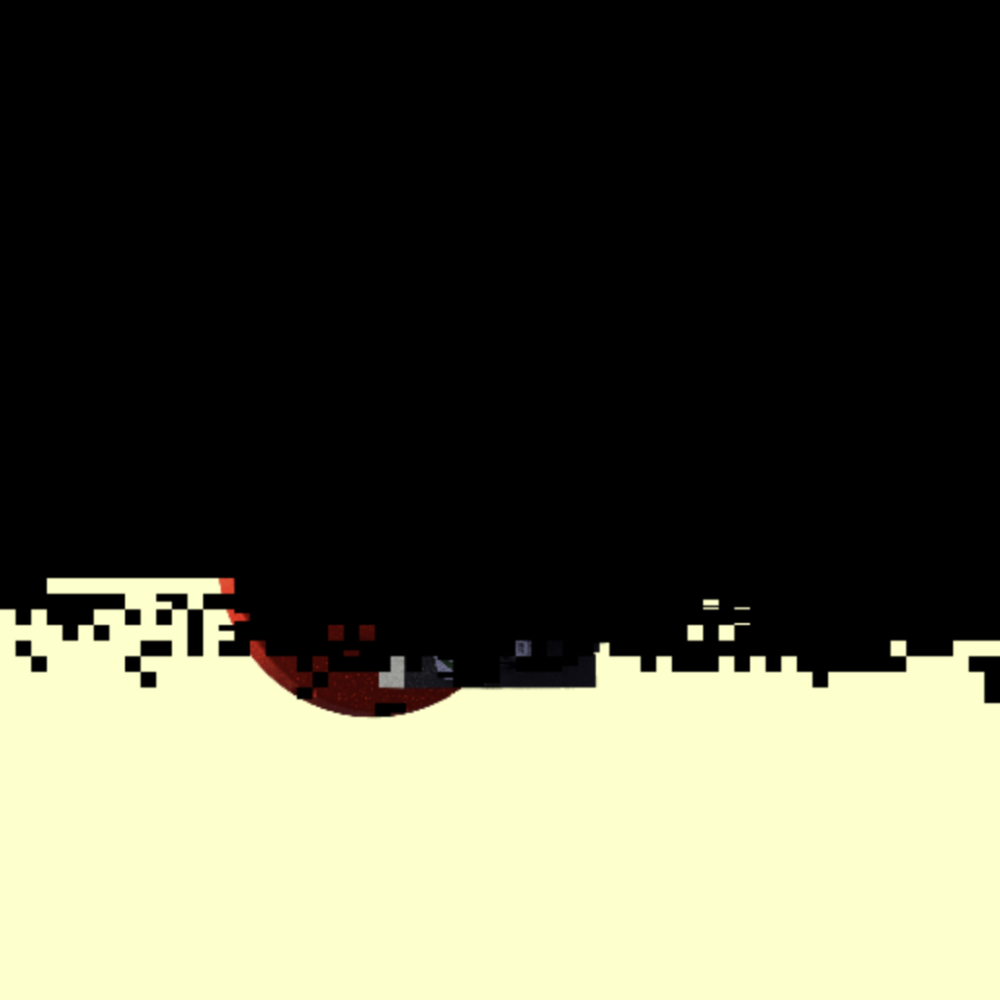
\includegraphics[width=0.25\columnwidth]{resources/webgpu-crashes.png}
  \caption{Example of a provoked WebGPU crash on macOS; note the black squares which correspond in size to the dispatched workgroup size.}
  \label{fig:webgpu-crash}
\end{figure}

\subsection*{OpenPBR}

The integration of the \gls{OpenPBR} surface shading model enables realistic material representation. As it is a new standard, and no stable version was released when implementation started, aligning the path tracer with the standard was challenging. After the standard reached a stable version, the alignment effort between the implementation and the standard was reduced.

To date, only a few open-source projects have implemented the standard. Neither \gls{Three.js} nor \gls{Babylon.js} have direct \gls{OpenPBR} support. However, there is a \gls{MaterialX} loader for \gls{Three.js} that could be used. For use in real-time rendering, alignment between \gls{OpenPBR} and \gls{glTF} \gls{PBR} extensions could be beneficial. This alignment could reduce the computational resources required for surface shading and improve interoperability by establishing \gls{glTF} extensions for \gls{OpenPBR}.

Using \gls{PBR} and the latest industry standards is beneficial and provides high-quality results. The adoption track of \gls{OpenPBR} is promising, and initiatives such as NVIDIA's \gls{OpenPBR} material library \cite{omniverseOpenPBR} can facilitate material creation. The standard is likely to be extended in the future. Such extensions could be specifications to support hair or volumetric effects.

\section{Future Work}

In order to accommodate other use cases, the renderer could be extended in various ways. The following section outlines possible future work, which includes extending \gls{PBR} capabilities, improving performance, extending to other rendering architecture paradigms, general improvements for the \gls{WebGPU} community, and aligning the renderer with other standards.

\subsection*{Rendering Improvements}

The focus on the defined use case means that certain rendering effects are not implemented. These include:

\begin{itemize}
    \item{Volumetric Effects}
    \item{Hair and Fur}
    \item{Refraction}
    \item{Caustics}
    \item{Depth of Field} — Effect of objects at different distances from the camera being in focus or out of focus.
    \item{Motion Blur} — Effect of objects moving quickly appearing blurred.
\end{itemize}

While refraction, caustics, depth of field, and motion blur are questions of light transport, volumetric effects, hair and fur are features that are not part of the \gls{OpenPBR} specification. Other features in terms of rendering could be implemented. This section outlines some of the possibilities.

\subsubsection*{Spectral Rendering}

Instead of using \gls{RGB} color space, spectral rendering could leverage the full spectrum of visible light by modeling the light as a function of wavelength. This can improve the realism of the rendered images. Spectral rendering is well-suited for \gls{PBR} and is a natural extension of the current implementation. It is also possible to support both \gls{RGB} and spectral rendering.

\subsubsection*{Texture Support}

While not critical for the given use case, texture support is a common feature in rendering engines. The current implementation does not use textures. The renderer could be extended to support sampling \gls{OpenPBR} parameters from textures. This would enable more complex material variations and improve the realism of the rendered images.

This is distinct from texture mapping frequently used in rasterization-based rendering engines. Texture mapping is a technique that applies images to surfaces to simulate surface details. In \gls{PBR}, textures are used to sample material properties such as base color, roughness, or metallicness.

\subsubsection*{Environment Mapping}

The current implementation offers a environment light setup. However, no details about the environment are visible in the reflections. By adding environment mapping, more complex lighting scenarios can be achieved. This could be done by using a skybox or a \gls{HDR} environment map.

\subsubsection*{Full OpenPBR support}

The current implementation only supports the \gls{OpenPBR} surface shading model features that are required for the given use case. The full \gls{OpenPBR} specification includes additional features that could be implemented to improve the realism of the rendered images. These include:

\begin{itemize}
  \item{Coat} - Secondary layer of specular highlight, often used for car paint.
  \item{Fuzz} – Layer for fuzzy or dusty surfaces.
  \item{Thin-film iridescence} - Effect of thin-films of material on the surface of an object. This can be seen in objects covered in grease, oil, or alcohol.
  \item{Subsurface Scattering and Translucency}
  \item{Opacity and Transparency}
\end{itemize}

\subsection*{Technical Improvements}

The renderer uses \gls{GPU} parallelization to accelerate the rendering process. However, the current implementation is not optimized for performance. This includes possible improvements on the \gls{CPU} and \gls{GPU} sides and the data transfer between the two. The following sections outline possible improvements and extensions of the current setup.

\subsubsection*{TypeScript Support for Memory Management}

While \texttt{webgpu-utils} \cite{webgpuUtilsLib} is helpful for memory management, it does not provide TypeScript support for the generated definitions based on the underlying \gls{WGSL} code. Type safety could reduce the likelihood of errors in the code. As an alternative, runtime checks could be implemented to ensure the data is correctly mapped to all fields of the underlying structure.

\subsubsection*{Web Worker Support}

Web Workers are a web technology that allows to run scripts off the main thread. This can be used to offload \gls{CPU}-heavy tasks to a separate thread to prevent blocking the main thread, which is responsible for rendering the user interface.

\subsubsection*{BVH Construction}
\label{sec:bvhConstructionDiscussion}

The current implementation builds the \gls{BVH} on the \gls{CPU} and transfers it to the \gls{GPU}. Corresponding research \cite{lauterbach2009GPUbvh} suggests that moving parts of the construction to the \gls{GPU} directly could improve performance. This would reduce the amount of data that needs to be transferred between the \gls{CPU} and the \gls{GPU}. The new \gls{GPGPU} capabilities of \gls{WebGPU} further enable this approach.

\subsubsection*{Independence of Three.js}

For ease-of-use for developers, the renderer uses \gls{Three.js} helpers. This aids developers familiar with \gls{Three.js} in getting started with the renderer, as the configuration for scene loading and camera configuration is similar. However, the renderer does not depend on \gls{Three.js} and could be used independently. The main drawback of the dependence is the increased bundle size. \texttt{three-mesh-bvh} \cite{threeMeshBvh} could also be exchanged for an alternative library. By removing the dependency, the bundle size would be reduced. To support developers, a binding to \gls{Three.js} could be provided on top of the independent renderer.

\subsubsection*{Offline and Remote Rendering}

As highlighted in \autoref{ch:paradigmAssessment}, it is possible to extend a real-time client-side renderer for offline and remote rendering scenarios. In order to implement offline rendering, one could opt to use a headless browser such as \texttt{Puppeteer}, a \fgls{Node.js}{JavaScript runtime, frequently used for executing JavaScript outside of the browser} library that provides a high-level \gls{API} to control browsers. An alternative is to use \gls{wgpu}, but this would necessitate a rewrite of the renderer. Possibly, the rewritten renderer could also be used in the web context by using \fgls{WebAssembly}{Portable Binary-code format for executable programs available in modern browser engines}.

For remote rendering, the renderer could be extended to render images on demand and encode them as video streams.

\subsubsection*{WebGPU Compatibility Mode}

There is a proposal under active development that aims to extend the reach of \gls{WebGPU} by providing a slightly restricted subset of \gls{WebGPU} \cite{WebGPUCompatibilityModeProposal}. Considering the suggested limits of the compatibility mode, it could be possible to deploy the renderer onto a broader range of devices. However, it is important to consider that path tracing is a computationally expensive task and might not be suitable for all devices. Therefore, increasing the reach might only be beneficial in some cases.

\subsubsection*{Automatic Shader Conversion}

During the specification phase of \gls{WebGPU}, the relation to \fgls{SPIR-V}{\e{Standard Portable Intermediate Representation}, intermediate language for parallel computing and graphics developed by Khronos Group} was discussed \cite{webGPUSpirVRelation}. In general, many of the modern shading languages can be compiled to one another. Projects such as \texttt{Tint}, which is part of \gls{Dawn} \cite{dawnImplementation} or \texttt{Naga} \cite{nagaImplementation} could be used to compile shaders from different frontends to different backends. Similarly, other engines, such as \gls{Three.js} with \fGls{TSL}{\e{Three.js Shading Language}, shading language used in \gls{Three.js} which supports \gls{GLSL} as well as \gls{WGSL}}, have their own shading languages that support a variety of backends \cite{ThreeJSShadingLanguage}. Parts of \gls{MaterialX} shader generation could be used to generate shaders for \gls{WebGPU} and update them automatically as \gls{OpenPBR} is updated.

\subsubsection*{Low-Level Performance Optimizations}

The current implementation is not optimized for performance. Therefore, optimizing the \gls{WGSL} code could improve the performance of the renderer. Due to the nature of the design of \gls{OpenPBR}, it would be possible to optimize and improve real-time rendering performance. One approach to do so is to establish so-called wavefront path tracing \cite{laine2013megakernels}. Instead of a single megakernel, the renderer could be split into multiple smaller kernels. One kernel would be responsible for ray generation, another for intersection testing, and multiple kernels for shading - one per workflow. This would reduce the divergence of the shader programs and could improve performance. Further investigation of potential performance improvements is required \cite{wavefrontComparisonInTableA5,mitsubaWavefrontVsMegakernel}.

This objective may be incompatible with the goal of providing automatic shader generation. Automatic shader generation is helpful but likely not as optimized as a carefully tuned implementation. However, both endeavors are of interest for potential benefits.

\subsection*{Quality Improvements}

This section highlights changes to improve the quality of the rendered images, reduce the amount of samples required, and enable better comparison of the renderer to baseline renderers.

\subsubsection*{Sampling Performance Optimizations}

Path tracing is computationally expensive and requires multiple samples per pixel to achieve accurate results. Consequently, the sampling process is noticeable during interactions with the scene. One technique to improve perceived interaction quality is to overlay the rendering with a rasterization preview during interactions. To reduce the number of samples required for high-quality renderings, techniques like neural radiance caching (NRC) \cite{muller2021real} or \gls{ReSTIR} \cite{restir} could be employed in future work.

\subsubsection*{Denoisers}

The renderer currently provides two optional strategies for denoising: \gls{OIDN} \cite{openImageDenoise} and Gaussian filtering. However, the quality of the results varies depending on the scene. In certain setups, the changes introduced by \gls{OIDN} are rather pronounced, which may necessitate disabling the denoiser. By employing alternative denoising algorithms, applied as post-processing steps, the quality of the results could be enhanced without introducing new artifacts into the renderings. Options include blockwise multi-order feature regression (BMFR) \cite{blockwise-multi-order-regresssion-for-rt-pt} and non-local means (NLM) denoising \cite{buadesNLMDenoising}.

\subsubsection*{Qualitative Assessment}

The provided results highlight the quantitative performance of the renderer. However, due to the nature of a renderer, qualitative assessment based on visual inspection is also used to determine the quality of the rendered images. This could be extended to include more advanced metrics such as peak signal to noise ratio (PSNR), structural similarity (SSIM) \cite{ssim}, or learned perceptual image patch similarity (LPIPS) \cite{lpips}.

Such a comparison could be based on reference scenes such as the Cornell Box \cite{goral1984modeling} or the Sponza Atrium \cite{dabrovic2002sponza}. To assess the differences, different comparisons could be conducted:

\begin{itemize}
    \item{Offline Renderer} - Comparison to other offline renderers such as Mitsuba \cite{Jakob2020DrJit}, \gls{pbrt} \cite{Pharr_Physically_Based_Rendering_2023}, or Cycles which is used by \gls{Blender} \cite{cycles}.
    \item{Rasterization Renderer} - Comparison to rasterization-based web renderers such as \gls{Three.js} or \gls{Babylon.js}.
    \item{Web-based Path Tracer} - Comparison to other web-based path tracers such as \texttt{three-gpu-pathtracer} \cite{ThreeJsPathTracerJohnson}, \texttt{Three.js PathTracer} \cite{ThreeJsPathTracerLoftis}, or \texttt{dspbr-pt} \cite{PathTracerDassault}.
\end{itemize}

\section{Conclusion}

While there are a variety of areas to improve on, the proposed solution constitutes a fully functional path tracer encompassing technical features such as using \gls{BVH}, parallelization on \gls{GPU} based on \gls{WebGPU}, and supporting \gls{MIS}; rendering features including anti-aliasing, denoising options, tone mapping, generating a wide range of global illumination effects, and supporting the \gls{OpenPBR} standard; usability features such as incremental rendering, camera controls, and scene loading; benchmarking setup for reliable performance measurements; and extensive documentation to facilitate use of the renderer.

These features fulfil the requirements of the use case and present an alternative to existing offline rendering solutions by permitting a higher degree of interactivity and alleviating the need to pregenerate all images, which facilitates offering more complex product families. Compared to remote rendering services, the approach reduces infrastructure cost and network dependency. The fidelity gained by using ray tracing techniques in combination with the \gls{OpenPBR} standard provides a high-quality rendering solution without the need for pregenerated assets. The path tracer developed in this thesis is a suitable choice for the given use case of using production \gls{CAD} data with manifold assembly configurations and customer-specific materials.

As shown in \autoref{sec:benchmark}, the performance is sufficient for near real-time renderings of assembled \gls{CAD} models on the web. The use of \gls{WebGPU} over \gls{WebGL} as well as incorporating \gls{OpenPBR} provides a distinction to existing open-source path tracers for the web. \gls{WebGPU} has significant potential for the years to come and adoption of \gls{OpenPBR} by the wider industry is a promising sign of the possible longevity of the chosen technology and standards. The open-source nature of the project facilitates extension and serves as inspiration for future initiatives.
